\begin{center}
    \begin{large}
    Cp 5 - Clases\\
    Curso \academicyear\\
    \end{large}
    \begin{figure}[h]
    	\centering
    	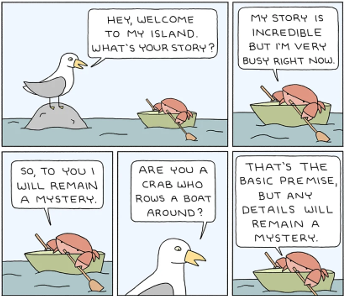
\includegraphics[width=0.5\linewidth]{cp5/classes.png}
    \end{figure}
\end{center}

% \section{MyList}
% Implemente la clase \textcolor{cyan}{MyList} para representar una lista de enteros. 

\subsection*{Funcionalidades a Implementar}
\begin{itemize}
    \item \textbf{Obtener el número de elementos (\texttt{Count})}: 
     Propiedad que devuelve el número de elementos en la lista.
    
    \item \textbf{Añadir un elemento (\texttt{Add})}:
     Método para añadir un elemento a la lista.
    
    \item \textbf{Vaciar la Lista (\texttt{Clear})}:
    Método para eliminar todos los elementos de la lista.
    
    \item \textbf{Verificar contenido (\texttt{Contains})}:
    Método que comprueba si un elemento está presente en la lista.
     
    \item \textbf{Obtener el Índice de un Elemento (\texttt{IndexOf})}:
    Método que devuelve el índice de la primera aparición de un elemento específico en la lista.
    
    \item \textbf{Insertar en un Índice Específico (\texttt{Insert})}:
    Método para insertar un elemento en un índice específico de la lista.
    
    \item \textbf{Eliminar un Elemento (\texttt{Remove})}:
    Método para eliminar la primera aparición de un elemento específico de la lista.
    
    \item \textbf{Eliminar en un Índice Específico (\texttt{RemoveAt})}:
    Método para eliminar el elemento en un índice específico de la lista.
    
    \item \textbf{Acceder a un Elemento por Índice (\texttt{this[int index]})}:
    Propiedad indexadora que permite acceder a los elementos de la lista mediante su índice.
\end{itemize}

\textbf{Ejemplo de uso:}
\begin{lstlisting}
// Crear una instancia de MyList
MyList myList = new MyList();

// Añadir elementos a la lista
myList.Add(10);
myList.Add(20);
myList.Add(30);
Console.WriteLine("Count: " + myList.Count);
// Esperado: Count: 3

// Acceder a elementos por índice
Console.WriteLine("Elemento en índice 1: " + myList[1]);
// Esperado: Elemento en índice 1: 20

// Verificar si un elemento está en la lista
bool contains = myList.Contains(20);
Console.WriteLine("¿Contiene 20?: " + contains);
// Esperado: ¿Contiene 20?: True

// Obtener el índice de un elemento
int index = myList.IndexOf(30);
Console.WriteLine("Índice de 30: " + index);
// Esperado: Índice de 30: 2

// Insertar un elemento en un índice específico
myList.Insert(1, 15);
Console.WriteLine("Elemento en índice 1 después de Insert: " + myList[1]);
// Esperado: Elemento en índice 1 después de Insert: 15

// Eliminar un elemento por valor
myList.Remove(20);
Console.WriteLine("¿Contiene 20 después de Remove?: " + myList.Contains(20));
// Esperado: ¿Contiene 20 después de Remove?: False

// Eliminar un elemento por índice
myList.RemoveAt(0);
Console.WriteLine("Elemento en índice 0 después de RemoveAt: " + myList[0]);
// Esperado: Elemento en índice 0 después de RemoveAt: 15

// Vaciar la lista
myList.Clear();
Console.WriteLine("Count después de Clear: " + myList.Count);
// Esperado: Count después de Clear: 0
\end{lstlisting}


\section{Fracción}
Implemente una clase llamada \textcolor{cyan}{Fraction} para representar el comportamiento de una fracción. Una fracción consta de dos enteros, el numerador y el denominador, donde el denominador no puede ser cero. Dos fracciones se consideran iguales si la relación entre el numerador y el denominador es la misma (por ejemplo, $\frac{1}{2}$ y $\frac{2}{4}$ son equivalentes).

\subsection*{Funcionalidades a implementar}
\begin{itemize}
    \item \textbf{Obtener el numerador (simplificado)}: Devuelve el numerador de la fracción en su forma simplificada.
    \item \textbf{Obtener el denominador (simplificado)}: Devuelve el denominador de la fracción en su forma simplificada.
    \item \textbf{Representación en cadena de caracteres}: Devuelve una cadena que representa la fracción en el formato \texttt{num/den} (por ejemplo, \texttt{1/2}).
    \item \textbf{Suma de fracciones}: Realiza la suma de dos fracciones y devuelve el resultado como una nueva fracción.
    \item \textbf{Resta de fracciones}: Resta una fracción de otra y devuelve el resultado como una nueva fracción.
    \item \textbf{Multiplicación de fracciones}: Multiplica dos fracciones y devuelve el resultado como una nueva fracción.
    \item \textbf{División de fracciones}: Divide una fracción por otra y devuelve el resultado como una nueva fracción.
    \item \textbf{Comparación de fracciones}: Permite comparar dos fracciones para determinar si una es menor, mayor o igual a la otra.
\end{itemize}

\textbf{Ejemplo de uso:}
\begin{lstlisting}
Fraction f1 = new Fraction(2, 4);
Fraction f2 = new Fraction(1, 3);

// Suma de fracciones
Fraction sum = f1 + f2;
Console.WriteLine(sum.ToString());
// Esperado: 5/6

// Resta de fracciones
Fraction diff = f1 - f2;
Console.WriteLine(diff.ToString());
// Esperado: 1/6

// Multiplicación de fracciones
Fraction product = f1 * f2;
Console.WriteLine(product.ToString());
// Esperado: 1/6

// División de fracciones
Fraction quotient = f1 / f2;
Console.WriteLine(quotient.ToString());
// Esperado: 3/2

// Comparación de fracciones
bool isEqual = f1 == f2;
Console.WriteLine(isEqual);
// Esperado: False
\end{lstlisting}

\ifshowanswers
\section*{Respuesta:}
\lstinputlisting{cp5/code/Fraction.cs}
\fi

\section{Polinomio}
Implemente una clase \textcolor{cyan}{Poly} para representar el comportamiento de un polinomio. Para representar un polinomio de grado n con coeficientes enteros se puede usar un array, de tal manera que en la posición k del array esté el coeficiente de grado k del polinomio. Así, para representar al polinomio \(p(x)=2 x+1\) se puede usar el array \([1,2]\) y para representar al polinomio \(p(x)=x^3-5x+1\) se puede usar el array \([1,-5,0,1]\).

\subsection*{Funcionalidades a implementar}

\begin{itemize}
    \item \textbf{Obtener el grado del polinomio}: Método que devuelve el grado del polinomio (índice más alto con coeficiente no nulo).
    
    \item \textbf{Obtener el coeficiente de una potencia específica}: Método que recibe un exponente \(k\) y devuelve el coeficiente de \(x^k\). Si \(k\) es mayor que el grado del polinomio, debe devolver 0.
    
    \item \textbf{Obtener el string que representa al polinomio}: Método que construye una representación en texto del polinomio. Ejemplo: si el array de coeficientes es \([0, -2, 1]\), debe devolver el string \(x^2 - 2x\). Los términos con coeficiente 0 no deben mostrarse, y los signos de cada término deben manejarse correctamente.
    
    \item \textbf{Comparar dos polinomios}: Métodos para compara dos polinomios $==, !=, >=, >, <=, <$.
    
    \item \textbf{Sumar dos polinomios}: Método que recibe otro polinomio y devuelve un nuevo polinomio que es la suma de ambos.
    
    \item \textbf{Multiplicar dos polinomios}: Método que recibe otro polinomio y devuelve un nuevo polinomio que es el producto de ambos.
    
    \item \textbf{Multiplicar un polinomio por un escalar \(e\)}: Método que recibe un entero \(e\) y devuelve un nuevo polinomio resultante de multiplicar todos los coeficientes por \(e\).
    
    \item * \textbf{Dividir dos polinomios}: Método que realiza la división entre dos polinomios, devolviendo el cociente como polinomio.

     \item * \textbf{Resto de dividir dos polinomios}: Método que realiza la división entre dos polinomios, devolviendo el residuo como polinomio.
    
    \item \textbf{Evaluar el polinomio en \(x\)}: Método que recibe un valor \(x\) y devuelve el resultado de evaluar el polinomio en ese valor.
    
    \item \textbf{Derivar el polinomio}: Método que devuelve un nuevo polinomio resultante de la derivada del polinomio actual, aplicando la regla de derivación \(\frac{d(x^k)}{dx} = k \cdot x^{k-1}\).
\end{itemize}

\textbf{Ejemplo de uso:}
\begin{lstlisting}
Poly.Poly p1 = new Poly.Poly([ 1, -5, 0, 1, 0, 0 ]); // x^3 - 5x + 1
Poly.Poly p2 = new Poly.Poly([ 2, 3 ]); // 3x + 2

// Obtener grado del polinomio
Console.WriteLine($"Grado de p1: {p1.Degree}");
// Esperado: 3

// Obtener coeficiente de una potencia específica
Console.WriteLine($"Coeficiente de x^2 en p2: {p2[2]}");
// Esperado: 0

// Suma de polinomios
Poly.Poly sum = p1 + p2;
Console.WriteLine(sum.ToString());
// Esperado: x^3 - 2x + 3

// Resta de polinomios
Poly.Poly diff = p1 - p2;
Console.WriteLine(diff.ToString());
// Esperado: x^3 - 8x - 1

// Multiplicación de polinomios
Poly.Poly product = p1 * p2;
Console.WriteLine(product.ToString());
// Esperado: 3x^4 + 2x^3 - 15x^2 - 7x + 2

// Evaluación del polinomio en un valor específico
int result = p1.Evaluate(2);
Console.WriteLine(result);
// Esperado: -1

// Derivada del polinomio
Poly.Poly derivative = p1.Derivative();
Console.WriteLine(derivative.ToString());
// Esperado: 3x^2 - 5
\end{lstlisting}

\ifshowanswers
\section*{Respuesta:}
\lstinputlisting{cp5/code/Poly.cs}
\fi

\section{Conjunto}
Implemente la clase \textcolor{cyan}{Set} para representar el comportamiento de un conjunto de enteros. Un conjunto es una colección de elementos únicos, es decir, no repetidos.

\subsection*{Funcionalidades a implementar}
\begin{itemize}
    \item \textbf{Obtener la cardinalidad}: 
    Método que devuelve el número de elementos en el conjunto.
    
    \item \textbf{Añadir un elemento}: 
    Método que agrega un nuevo elemento al conjunto. Si el elemento ya existe, no debe ser agregado de nuevo.
    
    \item \textbf{Eliminar un elemento}: 
    Método que elimina un elemento específico del conjunto. Si el elemento no existe en el conjunto, no se realiza ninguna acción.
    
    \item \textbf{Vaciar el conjunto}: 
    Método que elimina todos los elementos del conjunto, dejándolo vacío.

    \item \textbf{Pertenencia}: 
    Método que verifica si un elemento específico está presente en el conjunto (\(x \in B\)).
    
    \item \textbf{Intersección}: 
    Método que devuelve un nuevo conjunto con los elementos comunes entre dos conjuntos (\(A \cap B\)).
    
    \item \textbf{Unión}: 
    Método que devuelve un nuevo conjunto con todos los elementos de dos conjuntos (\(A \cup B\)),
    
    \item \textbf{Diferencia}: 
    Método que devuelve un nuevo conjunto con los elementos de \(A\) que no están en \(B\) (\(A - B\)).
    
    \item \textbf{Subconjunto}: 
    Método que determina si un conjunto está contenido dentro de otro (\(A \subseteq B\)).
    
    \item \textbf{Igualdad}: 
    Método que compara si dos conjuntos son iguales (\(A = B\)), es decir, si tienen exactamente los mismos elementos.
\end{itemize}

\textbf{Ejemplo de uso}

\begin{lstlisting}
Set s1 = new Set();
s1.Add(1);
s1.Add(2);
s1.Add(3);

Set s2 = new Set([2, 3, 4]);

// Obtener cardinalidad
Console.WriteLine($"Cardinalidad de s1: {s1.Cardinality}");
// Esperado: Cardinalidad de s1: 3

// Agregar un elemento
s1.Add(4);
Console.WriteLine($"Cardinalidad de s1 después de agregar 4: {s1.Cardinality}");
// Esperado: Cardinalidad de s1 después de agregar 4: 4

// Eliminar un elemento
s1.Remove(2);
Console.WriteLine($"Cardinalidad de s1 después de eliminar 2: {s1.Cardinality}");
// Esperado: Cardinalidad de s1 después de eliminar 2: 3

// Pertenencia
bool contains = s2.Contains(3);
Console.WriteLine($"¿s2 contiene 3?: {contains}");
// Esperado: ¿s2 contiene 3?: True

// Intersección
Set intersection = Set.Intersection(s1, s2);
Console.WriteLine($"Intersección de s1 y s2: [{string.Join(", ", intersection.Elements)}]");
// Esperado: Intersección de s1 y s2: [3, 4]

// Unión
Set union = Set.Union(s1, s2);
Console.WriteLine($"Unión de s1 y s2: [{string.Join(", ", union.Elements)}]");
// Esperado: Unión de s1 y s2: [1, 2, 3, 4]

// Diferencia
Set difference = Set.Difference(s2, s1);
Console.WriteLine($"Diferencia de s2 y s1: [{string.Join(", ", difference.Elements)}]");
// Esperado: Diferencia de s2 y s1: [2]

// Vaciar
s1.Clear()
Console.WriteLine($"Cardinalidad de s1 después de vaciar: {s1.Cardinality}");
// Esperado: Cardinalidad de s1 después de vaciar: 0

// Subconjunto
bool isSubset = Set.IsSubset(s1, s2);
Console.WriteLine($"¿s1 es subconjunto de s2?: {isSubset}");
// Esperado: ¿s1 es subconjunto de s2?: True

// Igualdad
bool isEqual = s1 == s2;
Console.WriteLine($"¿s1 es igual a s2?: {isEqual}");
// Esperado: ¿s1 es igual a s2?: False
\end{lstlisting}

\ifshowanswers
\section*{Respuesta:}
\lstinputlisting{cp5/code/Set.cs}
\fi

\section{Entero grande}
Implemente una clase \textcolor{cyan}{BigInt} para representar números enteros no negativos potencialmente grandes (pueden tener más de 1000 cifras). Esta clase debe permitir realizar operaciones aritméticas básicas de forma precisa, sin limitarse al rango de tipos numéricos tradicionales.

\subsection*{Funcionalidades a implementar}
\begin{itemize}
    \item \textbf{Obtener representación en cadena de caracteres}: Devuelve el número como un \texttt{string} que representa el valor completo del entero grande.
    \item \textbf{Suma}: Implementa la suma de dos objetos \textcolor{cyan}{BigInt}.
    \item \textbf{Resta}: Calcula la diferencia entre dos \textcolor{cyan}{BigInt}. \textbf{Nota:} asegúrese de que no se permitan resultados negativos.
    \item \textbf{Multiplicación}: Realiza la multiplicación entre dos objetos \textcolor{cyan}{BigInt}.
    \item * \textbf{División}: Implementa la división entre dos \textcolor{cyan}{BigInt}, devolviendo solo la parte entera del cociente.
    \item * \textbf{Resto de la división}: Calcula el residuo de la división entre dos \textcolor{cyan}{BigInt}.
    \item \textbf{Potenciación}: Permite elevar el número a una potencia \texttt{b} de tipo \texttt{int}.
    \item \textbf{Comparación}: Métodos para compara dos objetos \textcolor{cyan}{BigInt} $==, !=, >=, >, <=, <$.
\end{itemize}

\textbf{Ejemplo de uso:}
\begin{lstlisting}
BigInt bigInt1 = new BigInt("1000000000000000000000");
BigInt bigInt2 = new BigInt("100000000000000000000");

// Suma de enteros grandes
BigInt sum = bigInt1 + bigInt2;
Console.WriteLine(sum.ToString());
// Esperado: 1100000000000000000000

// Resta de enteros grandes
BigInt diff = bigInt1 - bigInt2;
Console.WriteLine(diff.ToString());
// Esperado: 900000000000000000000

// Multiplicación de enteros grandes
BigInt product = bigInt1 * bigInt2;
Console.WriteLine(product.ToString());
// Esperado: 100000000000000000000000000000000000000000

// Potenciación
int exponent = 2;
BigInt pow = BigInt.Pow(bigInt2, exponent);
Console.WriteLine(pow.ToString());
// Esperado: 10000000000000000000000000000000000000000

// Comparación de enteros grandes
Console.WriteLine(bigInt1 < bigInt2);
// Esperado: False
\end{lstlisting}

\ifshowanswers
\section*{Respuesta:}
\lstinputlisting{cp5/code/BigInt.cs}
\fi

\section{Fecha}
Implemente una clase llamada \textcolor{cyan}{Date} para representar una fecha, que incluya día, mes y año. Esta clase debe permitir realizar operaciones y consultas básicas sobre fechas.

\subsection*{Funcionalidades a implementar}
\begin{itemize}
    \item \textbf{Obtener el día}: Devuelve el día correspondiente de la fecha.
    \item \textbf{Obtener el mes}: Devuelve el mes correspondiente de la fecha.
    \item \textbf{Obtener el año}: Devuelve el año correspondiente de la fecha.
    \item \textbf{Obtener el día de la semana}: Calcula y devuelve el día de la semana en el que cae la fecha (por ejemplo, Lunes, Martes).
    \item \textbf{Comparar fechas}: Permite comparar dos fechas, indicando si una fecha es anterior, igual o posterior a otra.
    \item \textbf{Avanzar un día}: Ajusta la fecha actual avanzando un día, manejando correctamente los cambios de mes y año cuando sea necesario.
    \item \textbf{Retroceder un día}: Ajusta la fecha actual retrocediendo un día, manejando correctamente los cambios de mes y año cuando sea necesario.
    \item \textbf{Calcular la diferencia en días}: Calcula y devuelve la cantidad de días entre dos fechas dadas.
    \item \textbf{Representación en cadena de caracteres}: Devuelve la fecha en formato \texttt{día/mes/año} (por ejemplo, \texttt{12/10/2024}).
\end{itemize}

\textbf{Ejemplo de uso:}
\begin{lstlisting}
Date date1 = new Date(12, 10, 2024);
Date date2 = new Date(15, 10, 2024);

// Obtener el día, mes, año y el día de la semana
int day = date1.Day;                // Esperado: 12
int month = date1.Month;            // Esperado: 10
int year = date1.Year;              // Esperado: 2024
string dayOfWeek = date1.DayOfWeek; // Esperado: "Saturday"

// Comparar fechas con operadores
if (date1 < date2)
{
    Console.WriteLine($"{date1} es anterior a {date2}");
}
else if (date1 > date2)
{
    Console.WriteLine($"{date1} es posterior a {date2}");
}
else
{
    Console.WriteLine($"{date1} es igual a {date2}");
}
// Esperado: "12/10/2024 es anterior a 15/10/2024"

// Avanzar un día
date1.AdvanceOneDay();
Console.WriteLine(date1.ToString()); // Esperado: 13/10/2024

// Retroceder un día
date2.RetreatOneDay();
Console.WriteLine(date2.ToString()); // Esperado: 14/10/2024

// Calcular la diferencia en días entre dos fechas
int daysDifference = Date.DaysBetween(date1, date2);
Console.WriteLine($"Días de diferencia: {daysDifference}"); // Esperado: 1
\end{lstlisting}

\ifshowanswers
\subsection*{Hint:}
Reutiliza los métodos para fechas implementados en clase prácticas anteriores.
\fi

\section{Libro con reseñas}
Estamos desarrollando un sistema para gestionar una biblioteca digital que permita a los usuarios agregar reseñas y calificaciones a los libros, y necesitamos tu ayuda para implementar una clase que represente los libros en este sistema. Tu tarea es diseñar una clase \textcolor{cyan}{Book} que encapsule de manera segura toda la información de un libro.

\begin{itemize}
    \item \textbf{Propiedades (de solo lectura):}
    \begin{itemize}
        \item \texttt{Title} (string): el título del libro.
        \item \texttt{Author} (string): el nombre del autor.
        \item \texttt{Genre} (enum): el género del libro (Ficción, No Ficción, Ciencia, Historia, etc).
        \item \texttt{ISBN} (string): el identificador único del libro, que debe ser inmutable tras la creación del objeto.
    \end{itemize}
    
    \item \textbf{Métodos Públicos:}
    \begin{itemize}
        \item \texttt{AddReview(string reviewText, int rating)}: agrega una reseña al libro con un texto y una calificación (de 1 a 5).
        \item \texttt{GetReviews()}: devuelve todas las reseñas del libro como un solo string, mostrando el texto y la calificación de cada reseña, separadas por saltos de línea.
        \item \texttt{GetAverageRating()}: calcula y devuelve el promedio de todas las calificaciones de las reseñas.
        \item \texttt{GetSummary()}: devuelve un breve resumen del libro en el siguiente formato:
        \begin{verbatim}
    Title: [Título]
    Author: [Autor]
    Genre: [Género]
    ISBN: [ISBN]
        \end{verbatim}
    \end{itemize}
\end{itemize}

\textbf{Ejemplo de uso:}
\begin{lstlisting}
Book book = new Book("The Great Gatsby", "F. Scott Fitzgerald",
                     Genre.Fiction, "978-0743273565");
book.AddReview("Amazing classic!", 5); 
book.AddReview("A timeless tale of love and loss.", 4); 

Console.WriteLine(book.GetSummary()); 
// Esperado: 
// Title: The Great Gatsby
// Author: F. Scott Fitzgerald
// Genre: Fiction
// ISBN: 978-0743273565

Console.WriteLine("Reviews:");
Console.WriteLine(book.GetReviews()); 
// Esperado:
// Review 1: Amazing classic! (Rating: 5)
// Review 2: A timeless tale of love and loss. (Rating: 4)"

Console.WriteLine("Average Rating: " + book.GetAverageRating()); 
// Esperado: 
// Average Rating: 4.5
\end{lstlisting}


% \section{Número Complejo}
% Implemente una clase llamada \textcolor{cyan}{MyComplex} que represente el comportamiento de un número complejo, compuesto por una parte real y una parte imaginaria. Esta clase debe proporcionar métodos para realizar operaciones y obtener propiedades específicas de los números complejos.

\subsection*{Funcionalidades a implementar}
\begin{itemize}
    \item \textbf{Obtener la parte real}: Devuelve la parte real del número complejo.
    \item \textbf{Obtener la parte imaginaria}: Devuelve la parte imaginaria del número complejo.
    \item \textbf{Representación en cadena de caracteres}: Devuelve una cadena en el formato estándar “$a + bi$”, donde \texttt{a} es la parte real y \texttt{b} es la parte imaginaria.
    \item \textbf{Conjugado}: Calcula el conjugado del número complejo. Si el número es $z = a + bi$, su conjugado es:
    \[
    \overline{z} = a - bi
    \]
    \item \textbf{Módulo}: Calcula el módulo del número complejo, es decir, la distancia desde el origen en el plano complejo. Para $z = a + bi$, el módulo es:
    \[
    |z| = \sqrt{a^2 + b^2}
    \]
    \item \textbf{Ángulo (argumento)}: Calcula el ángulo del número complejo en radianes, medido desde el eje positivo de las abscisas. 
    % Para $z = a + bi$, el ángulo es:
    % \[
    % \theta = 
    % \begin{cases} 
    % \arctan\left(\frac{b}{a}\right) & \text{si } a > 0 \, (\text{Primer o Cuarto cuadrante}), \\
    % \arctan\left(\frac{b}{a}\right) + \pi & \text{si } a < 0 \text{ y } b \geq 0 \, (\text{Segundo cuadrante}), \\
    % \arctan\left(\frac{b}{a}\right) - \pi & \text{si } a < 0 \text{ y } b < 0 \, (\text{Tercer cuadrante}), \\
    % \frac{\pi}{2} & \text{si } a = 0 \text{ y } b > 0 \, (\text{Eje positivo imaginario}), \\
    % -\frac{\pi}{2} & \text{si } a = 0 \text{ y } b < 0 \, (\text{Eje negativo imaginario}), \\
    % 0 & \text{si } b = 0 \text{ y } a > 0 \, (\text{Eje positivo real}), \\
    % \pi & \text{si } b = 0 \text{ y } a < 0 \, (\text{Eje negativo real}).
    % \end{cases}
    % \]
    % Considerando el cuadrante correspondiente.
    \item \textbf{Suma de números complejos}: Realiza la suma de dos números complejos. Dados $z_1 = a + bi$ y $z_2 = c + di$, su suma es:
    \[
    z_1 + z_2 = (a + c) + (b + d)i
    \]
    \item \textbf{Resta de números complejos}: Calcula la diferencia entre dos números complejos. Dados $z_1 = a + bi$ y $z_2 = c + di$, su resta es:
    \[
    z_1 - z_2 = (a - c) + (b - d)i
    \]
    \item \textbf{Multiplicación de números complejos}: Realiza la multiplicación de dos números complejos. Dados $z_1 = a + bi$ y $z_2 = c + di$, su producto es:
    \[
    z_1 \cdot z_2 = (ac - bd) + (ad + bc)i
    \]
    \item \textbf{División de números complejos}: Realiza la división entre dos números complejos, devolviendo el resultado en forma de otro número complejo. Dados $z_1 = a + bi$ y $z_2 = c + di$, su división es:
    \[
    \frac{z_1}{z_2} = \frac{(ac + bd) + (bc - ad)i}{c^2 + d^2}
    \]
\end{itemize}

\textbf{Ejemplo de uso:}
\begin{lstlisting}
MyComplex c1 = new MyComplex(3, 4); // 3 + 4i
MyComplex c2 = new MyComplex(1, -2); // 1 - 2i

// Suma de números complejos
MyComplex sum = c1 + c2;
Console.WriteLine(sum.ToString());
// Esperado: 4 + 2i

// Resta de números complejos
MyComplex diff = c1 - c2;
Console.WriteLine(diff.ToString());
// Esperado: 2 + 6i

// Multiplicación de números complejos
MyComplex product = c1 * c2;
Console.WriteLine(product.ToString());
// Esperado: 11 - 2i

// División de números complejos
MyComplex quotient = c1 / c2;
Console.WriteLine(quotient.ToString());
// Esperado: -1.4 + 2.2i

// Conjugado de un número complejo
MyComplex conjugate = c1.Conjugate;
Console.WriteLine(conjugate.ToString());
// Esperado: 3 - 4i

// Módulo de un número complejo
double modulus = c1.Modulus;
Console.WriteLine(modulus);
// Esperado: 5 (porque sqrt(3^2 + 4^2) = 5)

// Ángulo (argumento) de un número complejo
double angle = c1.Argument;
Console.WriteLine(angle);
// Esperado: 0.9273 (en radianes)

// Comparación de igualdad
bool isEqual = c1 == c2;
Console.WriteLine(isEqual);
// Esperado: False
\end{lstlisting}


% \section{* Punto}
% Implementa una clase llamada \textcolor{cyan}{MyPoint} que contenga dos propiedades, \texttt{X} y \texttt{Y}, para almacenar las coordenadas de un punto en el plano.

\subsection*{Funcionalidades a implementar}
\begin{itemize}
    \item \textbf{Distancia entre puntos (\texttt{DistanceBetweenMyPoints})}: 
    Método que reciba dos objetos de tipo \textcolor{cyan}{MyPoint} y devuelva la distancia entre los dos puntos.
\end{itemize}

\subsection*{Métodos adicionales}
Implemente los siguientes métodos de manera externa a la clase \textcolor{cyan}{MyPoint}:
\begin{enumerate}
    \item \textbf{Promedio de distancias (\texttt{AverageDistance})}: 
    Método que recibe un array de objetos \textcolor{cyan}{MyPoint} y un punto de referencia. El método debe calcular y devolver el promedio de las distancias entre cada punto del array y el punto de referencia.

     \item \textbf{Verificar si los puntos están en una recta (\texttt{AreMyPointsCollinear})}: 
    Método que verifica si todos los puntos de un array de \textcolor{cyan}{MyPoint} se encuentran alineados en una única línea recta.

    \item \textbf{Puntos con menor distancia (\texttt{PointsWithMinDistance})}: 
    Método que, dado un array de objetos \textcolor{cyan}{MyPoint}, devuelve los dos puntos que están a la menor distancia entre sí.

    \item * \textbf{Ordenar por cercanía (\texttt{SortByProximity})}: 
    Método que recibe un array de objetos \textcolor{cyan}{MyPoint} y un punto de referencia. El método debe devolver un nuevo array en el que los puntos están ordenados en función de su proximidad al punto de referencia.

    \item * \textbf{Ordenar por cercanía en el lugar (\texttt{SortByProximityInPlace})}: 
    Método que modifica el array original de objetos \textcolor{cyan}{MyPoint}, ordenándolos por su proximidad al punto de referencia, sin generar un nuevo array.
\end{enumerate}


% \section{* Polígono}
% Implemente una clase llamada \textcolor{cyan}{Polygon} que reciba una secuencia de puntos en su constructor, representando los vértices del polígono.

\subsection*{Funcionalidades a implementar}
\begin{itemize}
    \item \textbf{Verificar si es un polígono cerrado (\texttt{IsPolygon})}: 
    Método que verifica si la secuencia de puntos constituye un polígono cerrado. Para esto:
    \begin{itemize}
        \item Asegúrese de que no haya tres puntos consecutivos alineados.
        \item Verifique que el primer punto coincida con el último para formar un cierre.
    \end{itemize}
    
    \item \textbf{Calcular el perímetro (\texttt{Perimeter})}: 
    Método que calcula la longitud total del contorno del polígono, sumando las distancias entre puntos consecutivos, incluyendo la distancia entre el último punto y el primero para cerrar el polígono.
    
    \item * \textbf{Calcular el área (\texttt{Area})}: 
    Método que calcula el área del polígono usando la fórmula para polígonos simples. Esta fórmula es válida tanto para polígonos convexos como cóncavos simples. La fórmula se basa en la suma de áreas de triángulos formados por los vértices del polígono.

    \item ** \textbf{Punto interior (\texttt{IsPointInside})}: 
    Método que verifica si un punto dado se encuentra dentro del polígono.
\end{itemize}

